\documentclass[spanish]{beamer}

%Language symbols
\usepackage[spanish]{babel}
\selectlanguage{spanish}
\usepackage[utf8]{inputenc}
\usepackage{verbatim}


\usepackage{graphicx}% http://ctan.org/pkg/graphicx
\usepackage{caption,subcaption}

% Code

\usepackage{listings,textcomp}
\lstset{
  breakatwhitespace,
  language=c++,
  columns=fullflexible,
  keepspaces,
  breaklines,
  tabsize=2, 
  showstringspaces=false,
  extendedchars=true,
  basicstyle=\fontfamily{pcr}\selectfont\scriptsize,
  keywordstyle=\color{orange},
  upquote=true,
  literate={-}{-}1}

%Theme
\usetheme{metropolis}

%Title
\title{Análisis de la eficiencia de algoritmos}
\date{\today}
\author{Yábir G. Benchakhtir}
\institute{Doble Grado en Ingeniería Informática y Matemáticas}
%Document
\begin{document}

\frame{\titlepage}

\begin{frame}\frametitle{Algoritmos a analizar}

  \begin{itemize}
  \item Burbuja
  \item Insercción
  \item Selección
  \item Mergesort
  \item Quicksort
  \item Heapsort
  \item Floyd 
  \item Hanoi
  \end{itemize}
\end{frame}

%
%======================
%

\begin{frame}\frametitle{Algoritmo burbuja}
  \begin{figure}[H]
    \centering   
        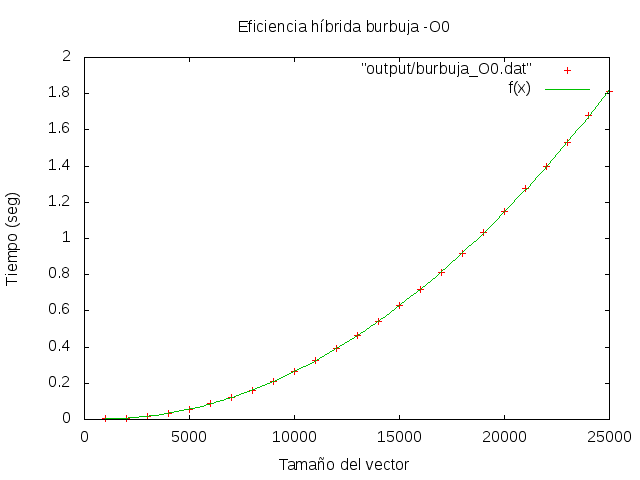
\includegraphics[clip,width=1\columnwidth]{../../plots/burbuja_O0_fit.png}%
    \end{figure}
  \end{frame}

\begin{frame}[fragile]
  Para su ajuste he usado la función:

  $$ax^2+bx+c$$
\scriptsize
\begin{verbatim}
final sum of squares of residuals : 9.84713e-05
Final set of parameters            Asymptotic Standard Error
=======================            ==========================

a               = 3.11154e-09      +/- 1.128e-11    (0.3624%)
b               = -5.17483e-06     +/- 3.02e-07     (5.837%)
c               = 0.00563209       +/- 0.001704     (30.26%)
\end{verbatim}
  
\end{frame}


%
%======================
%

\begin{frame}\frametitle{Algoritmo de inserción}
  \begin{figure}[H]
    \centering   
        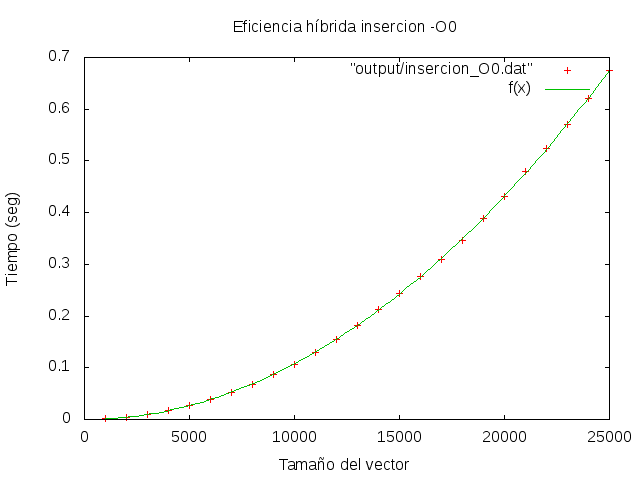
\includegraphics[clip,width=1\columnwidth]{../../plots/insercion_O0_fit.png}%
    \end{figure}
\end{frame}

\begin{frame}[fragile]
  Para su ajuste he usado la función:

  $$ax^2+bx+c$$
  
\scriptsize
\begin{verbatim}
final sum of squares of residuals : 7.19712e-05
Final set of parameters            Asymptotic Standard Error
=======================            ==========================

a               = 1.08271e-09      +/- 6.279e-12    (0.5799%)
b               = -7.7687e-08      +/- 1.682e-07    (216.5%)
c               = 0.000123925      +/- 0.0009489    (765.7%)
\end{verbatim}

\end{frame}


%
%======================
%

\begin{frame}\frametitle{Algoritmo de selección}
  \begin{figure}[H]
    \centering   
        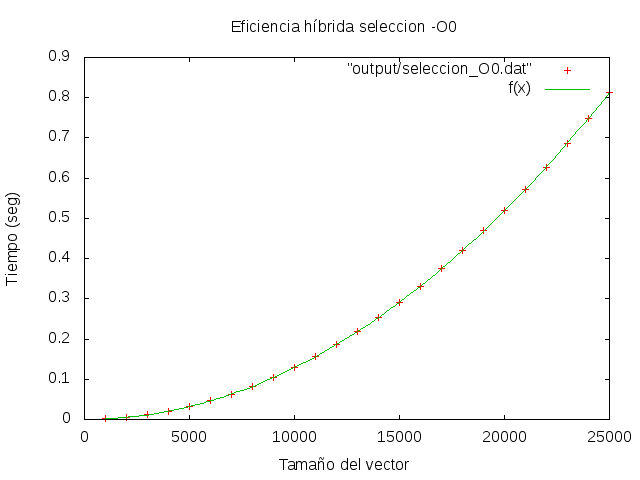
\includegraphics[clip,width=1\columnwidth]{../../plots/seleccion_O0_fit.png}%
    \end{figure}
  \end{frame}

\begin{frame}[fragile]
  Para su ajuste he usado la función:

  $$ax^2+bx+c$$
  
\scriptsize
\begin{verbatim}
final sum of squares of residuals : 8.779e-06
Final set of parameters            Asymptotic Standard Error
=======================            ==========================

a               = 1.30761e-09      +/- 1.868e-12    (0.1429%)
b               = -2.41748e-07     +/- 5.005e-08    (20.7%)
c               = 0.000572432      +/- 0.0002824    (49.33%)
\end{verbatim}
  
  
\end{frame}

%
%======================
%

\begin{frame}\frametitle{Comparación de los algoritmos}
  \begin{figure}[H]
    \centering   
        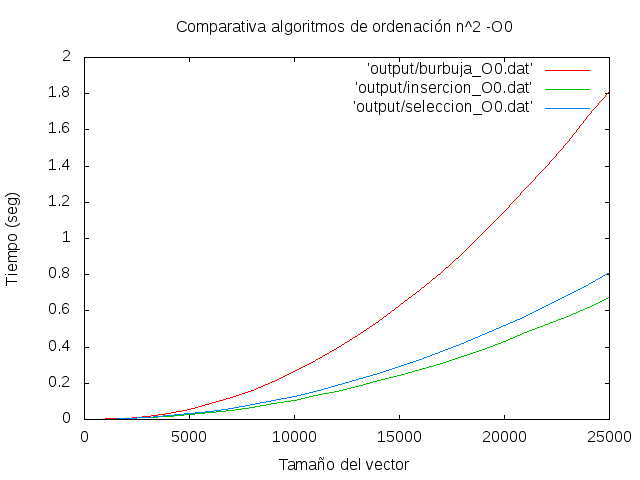
\includegraphics[clip,width=1\columnwidth]{../../plots/cuadraticos_O0.png}%
    \end{figure}
  \end{frame}

 \begin{frame}\frametitle{Mergesort}
    \begin{figure}[H]
    \centering   
    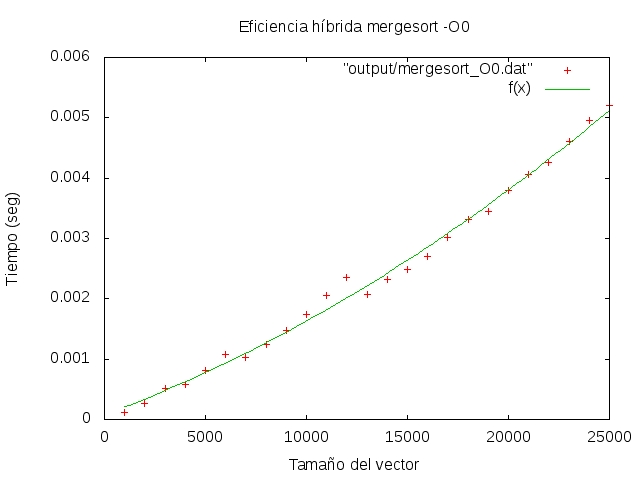
\includegraphics[clip,width=0.76\columnwidth]{../../plots/mergesort_O0_fit.png}%
    \end{figure}

    Para su ajuste he usado la función: $$ax\cdot log(bx +c)+d$$
       
  \end{frame}

   \begin{frame}\frametitle{Quicksort}
    \begin{figure}[H]
    \centering   
    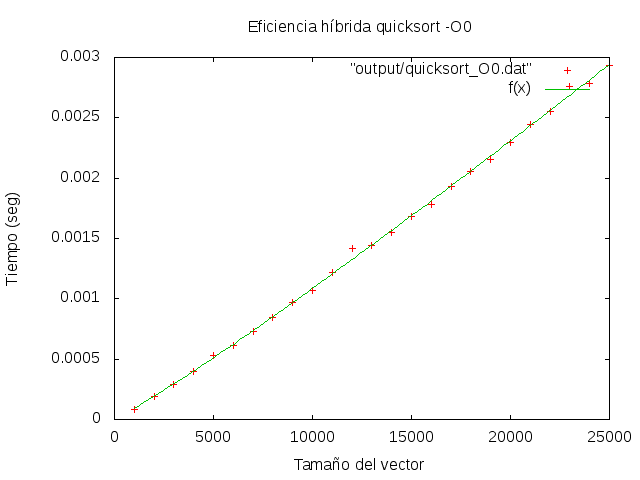
\includegraphics[clip,width=0.76\columnwidth]{../../plots/quicksort_O0_fit.png}%
    \end{figure}

    Para su ajuste he usado la función: $$ax\cdot log(bx +c)+d$$
       
  \end{frame}

   \begin{frame}\frametitle{Heapsort}
    \begin{figure}[H]
    \centering   
    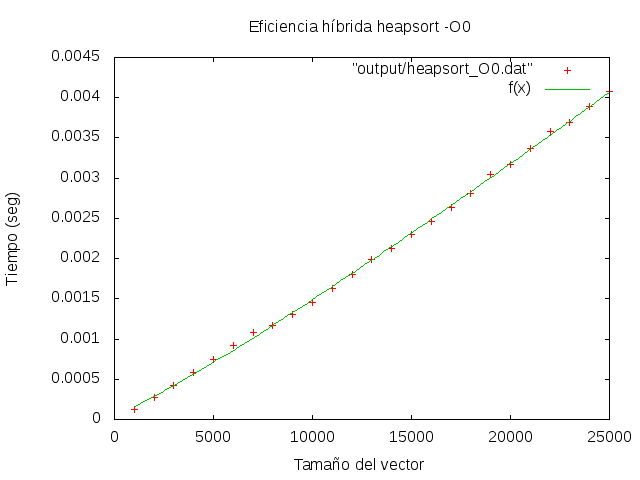
\includegraphics[clip,width=0.76\columnwidth]{../../plots/heapsort_O0_fit.png}%
    \end{figure}

    Para su ajuste he usado la función: $$ax\cdot log(bx +c)+d$$
       
  \end{frame}

\begin{frame}\frametitle{Comparación de los algoritmos $nlog(n)$}
  \begin{figure}[H]
    \centering   
        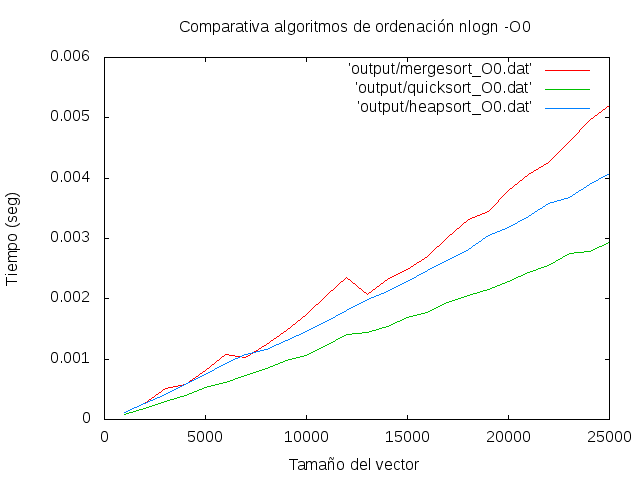
\includegraphics[clip,width=1\columnwidth]{../../plots/logaritmicos_O0.png}%
    \end{figure}
  \end{frame}



  

\begin{frame}\frametitle{Floyd}
  \begin{figure}[H]
    \centering   
        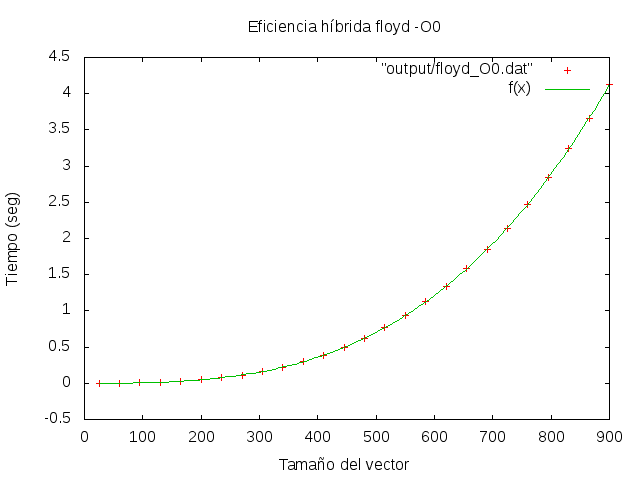
\includegraphics[clip,width=0.8\columnwidth]{../../plots/floyd_O0_fit.png}%
      \end{figure}

      Ajuste realizado con la función $f(x) = ax^3 + bx^2 + cx + d$
  \end{frame}
  
  \begin{frame}\frametitle{Hanoi}
    \begin{figure}[H]
      \centering   
      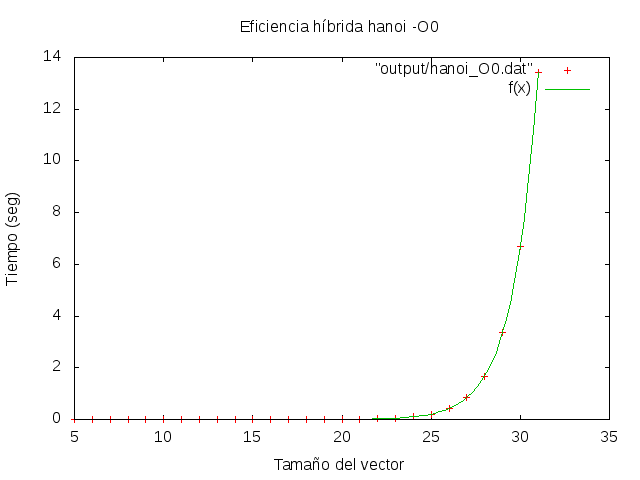
\includegraphics[clip,width=0.8\columnwidth]{../../plots/hanoi_O0_fit.png}%
    \end{figure}

    Ajuste realizado con la función $a2^x$
  \end{frame}

  
\begin{frame}\frametitle{Comparaciones usando otras eficiencias (burbuja)}
  \begin{figure}[H]
    \centering   
        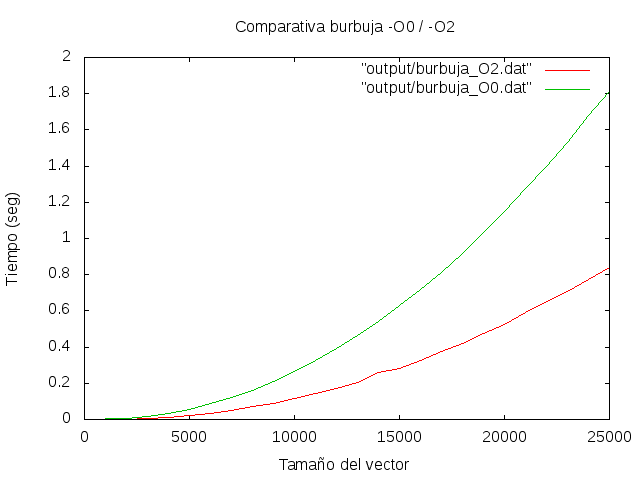
\includegraphics[clip,width=1\columnwidth]{../../plots/burbuja_comparativa.png}%
      \end{figure}
  \end{frame}

    
\begin{frame}\frametitle{Comparaciones usando otras eficiencias (hanoi)}
  \begin{figure}[H]
    \centering   
        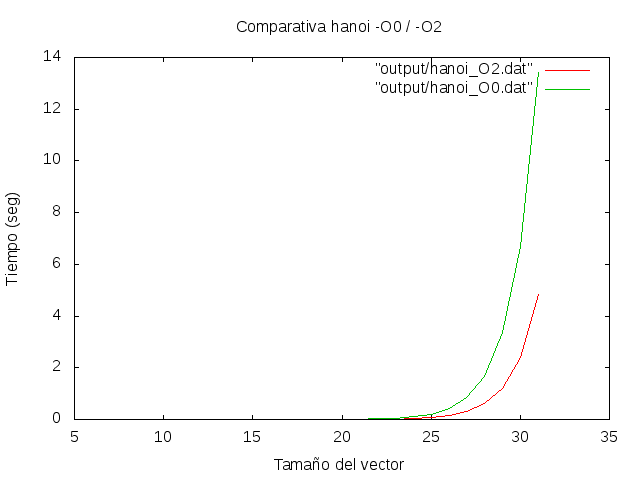
\includegraphics[clip,width=1\columnwidth]{../../plots/hanoi_comparativa.png}%
      \end{figure}
  \end{frame}

\end{document}

